\documentclass[12pt]{article}

\usepackage[utf8]{inputenc}
\usepackage{hyperref}
\usepackage{float} % To use 'H' for figures
\usepackage{graphicx} % for figure graphics
\usepackage[dvipsnames]{xcolor} % Text Colors
\usepackage{amssymb} % For 'mathbb'

\usepackage{amsmath}% http://ctan.org/pkg/amsmath

\usepackage{titlesec} % Title/Section Styling
\newcommand{\sectionbreak}{\clearpage} % Start each section from new page
\titleformat{\section} % Underline sections
  {\normalfont\Large\bfseries}{\thesection}{1em}{}[{\titlerule[0.8pt]}]


\setlength{\parindent}{0em}
\setlength{\parskip}{1em}

\title{Machine Learning: Supervised Methods
NOTES}
\author{Kristian Bonnici}


\begin{document}



\maketitle
\tableofcontents

\part{Theory}

\section{Introduction}

\subsection{Theoretical paradigms }\label{theoretical-paradigms}

Theoretical paradigms for machine learning \textbf{differ} mainly on
what they \underline{assume about the process generating the data}:

\begin{figure}[H]
  \centering  % Remember to centre the figure
    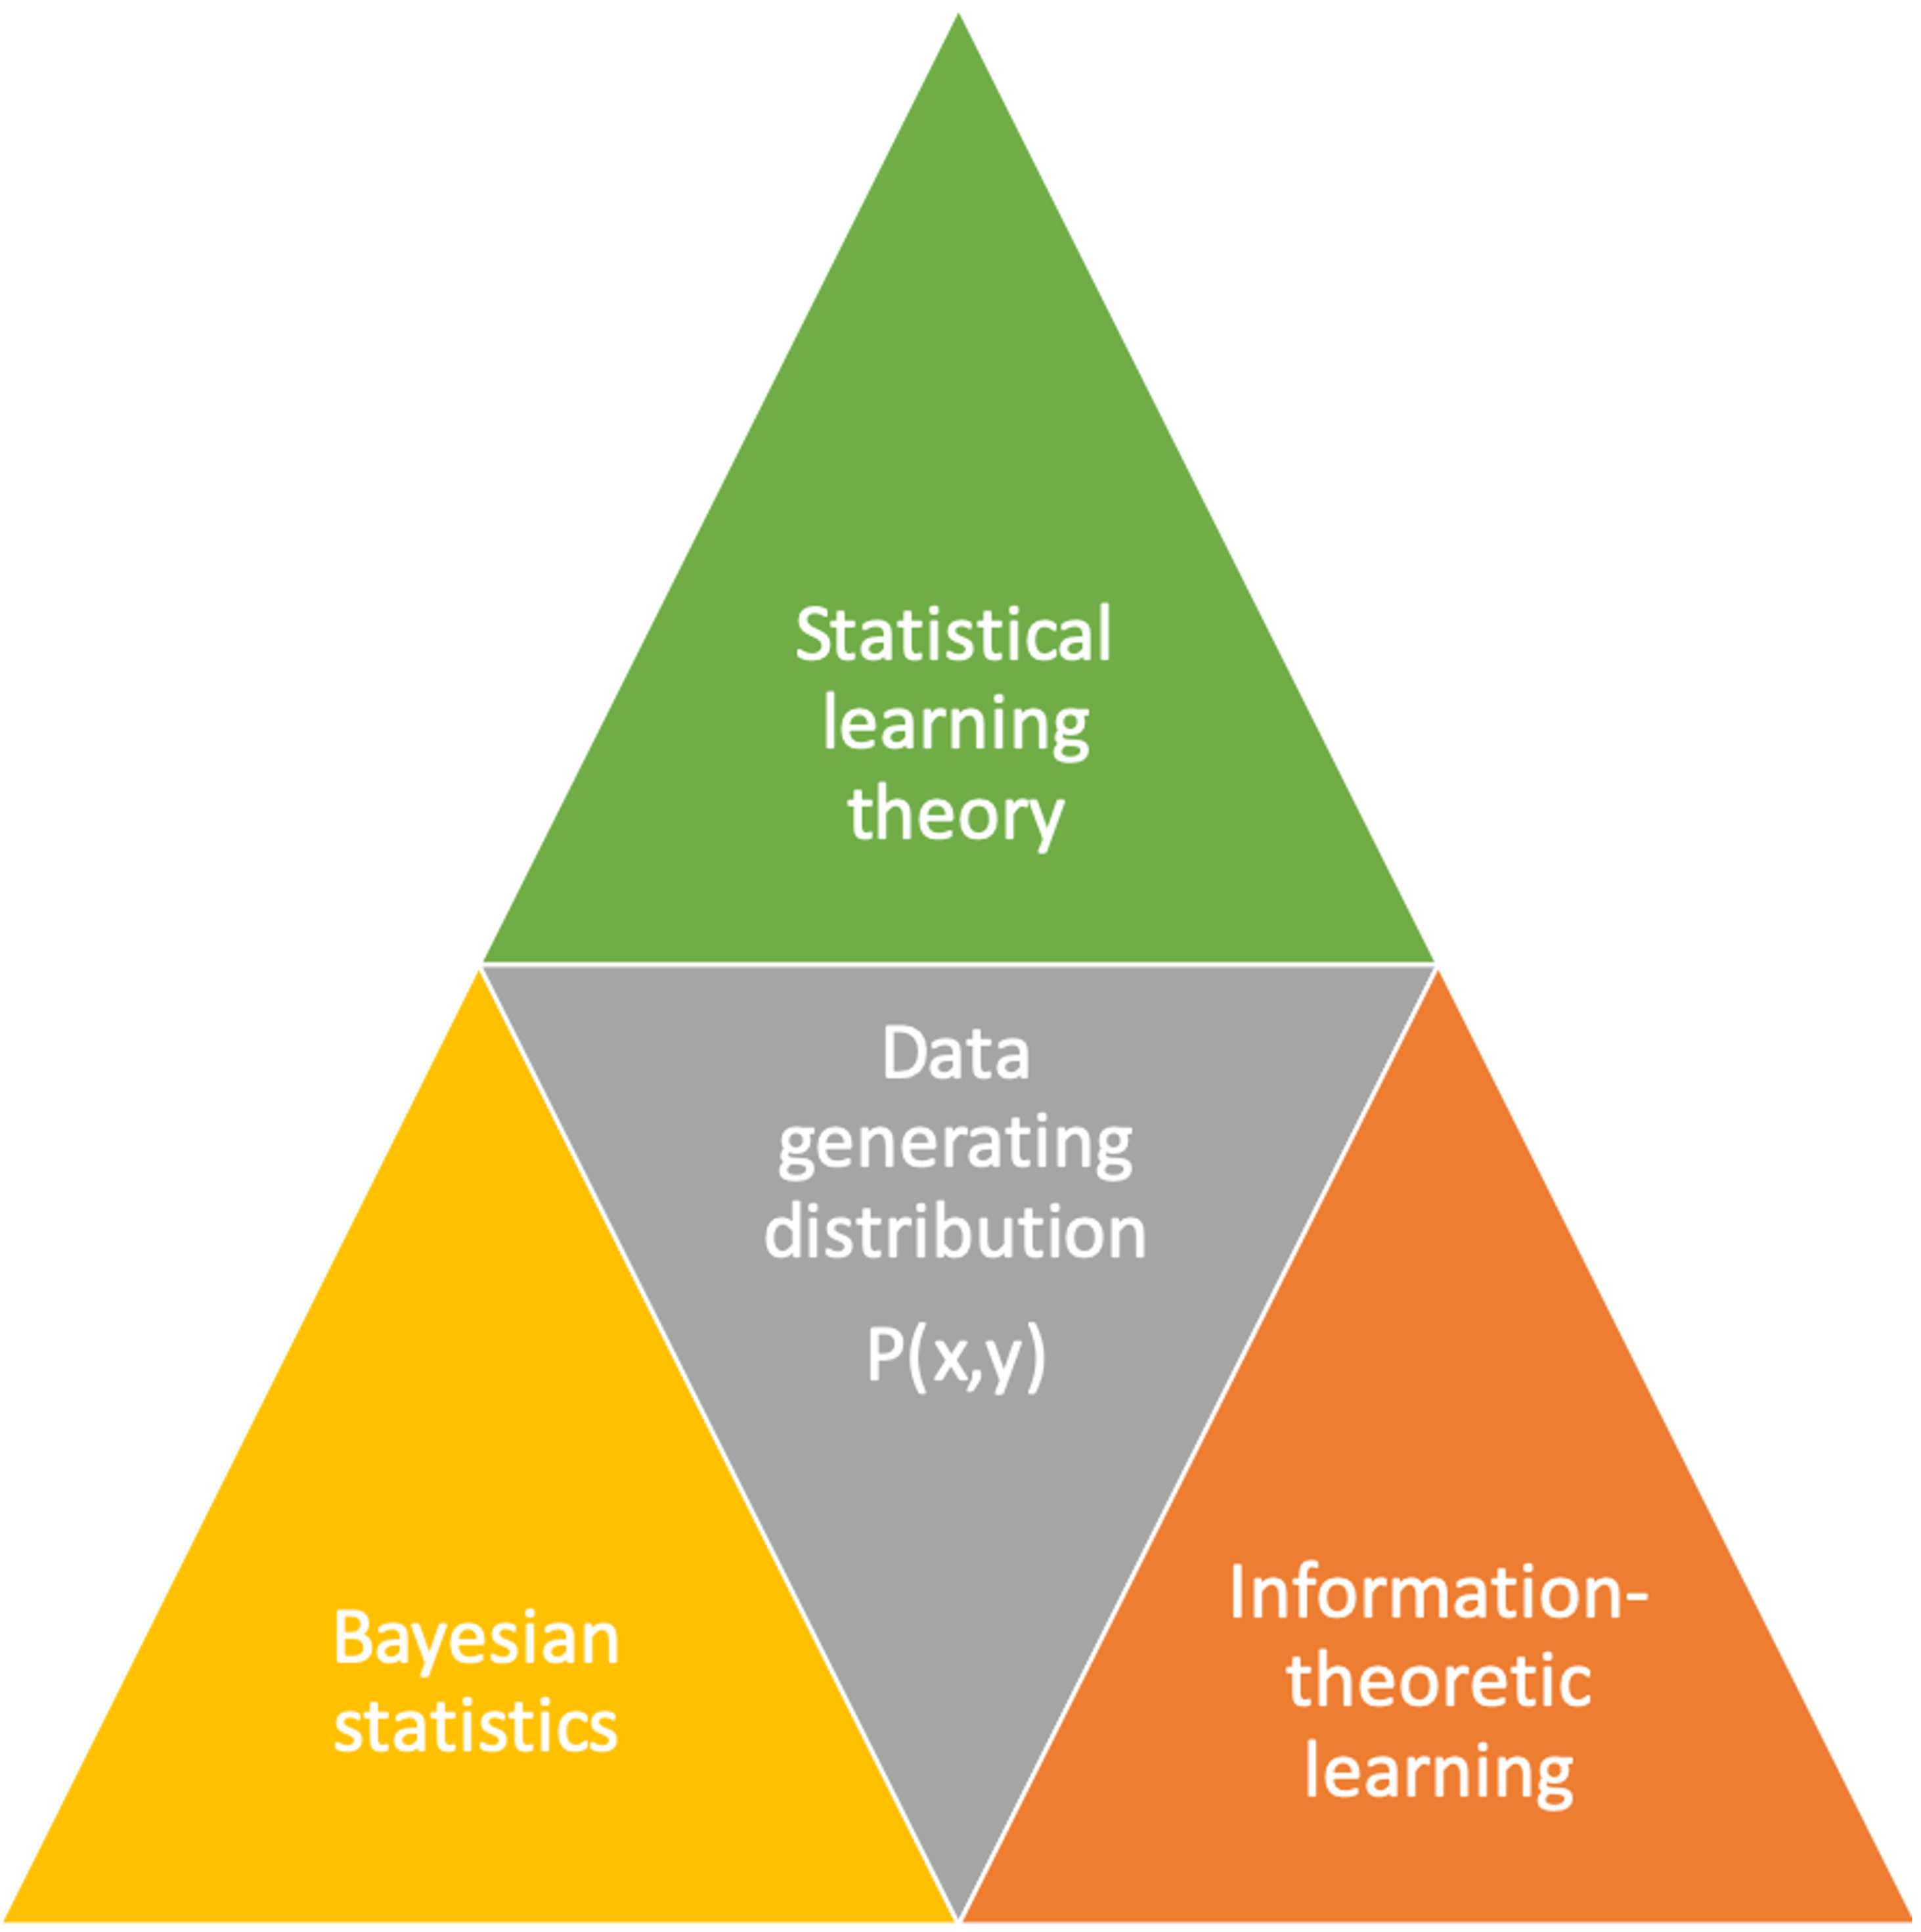
\includegraphics[width=0.5\columnwidth]{images/theoretical-paradigms.png}
    \caption{paradigms for data generation distributions.}
    \label{fig:fig1}
\end{figure}

\begin{itemize}
\item
  \textbf{\textcolor[HTML]{7EAA55}{Statistical learning theory (focus on this course)}:} assumes
  data is \underline{i.i.d} from an \underline{unknown distribution P(x)}, does not estimate the
  distribution (directly)
\item
  \textbf{\textcolor[HTML]{F5C342}{Bayesian Statistics}:} assumes \underline{prior information on P(x)}, estimates posterior probabilities
\item
  \textbf{\textcolor[HTML]{DE8344}{Information theoretic learning}:} (e.g.Minimum Description Length principle, MDL):
  estimates distributions, but does not assume a prior on P(x)

\end{itemize}

\subsection{Dimensions of a supervised learning algorithm
}\label{dimensions-of-a-supervised-learning-algorithm}

\begin{enumerate}
\def\labelenumi{\arabic{enumi}.}
\item
  \textbf{Training sample:} $S = \{(x_i, y_i)\}^m_{i=1}$ the training
  examples $(x, y) \in X \times Y$ independently drawn from a identical
  distribution $(i.i.d) D$ defined on $X \times Y, X$ is a space of inputs,
  $Y$ is the space of outputs.
\item
  \textbf{Model or hypothesis:} $h : X \rightarrow Y$ that we use to predict
  outputs given the inputs $x$.
\item
  \textbf{Loss function:} $L : Y \times Y \rightarrow \mathbb{R}, L(...) \geq 0, L(y, y')$ is the
  loss incurred when predicting $y'$ when $y$ is true.
\item
  \textbf{Optimization} procedure to find the hypothesis $h$ that
  minimize the loss on the training sample.
\end{enumerate}



\subsection{Classification (Task 1/3)}

\textbf{Problem:} partitioning the data into pre-defined classes by a
\emph{decision boundary} or \emph{decision surface}.

\textbf{Multi-class classification:} more than two classes

\begin{itemize}
  \item
    \textbf{Multi-label Classification:} An example can belong to multiple classes at the same time
  \item
    \textbf{Extreme classification:} Learning with thousands to
    hundreds of thousands of classes (Prof.~Rohit Babbar @ Aalto)
\end{itemize}



\subsubsection{Version space}\label{version-space}

\textbf{Version space:} the set of \underline{all \textcolor{blue}{consistent hypotheses}} of the
hypothesis class

\begin{itemize}
  \item
    \textbf{\textcolor{blue}{Consistent hypothesis}:} if correctly classifies all training
    examples
  \item
    \textbf{In version space:}
  \begin{itemize}
    \item
      \textbf{Most general hypothesis $G$:} cannot be expanded without
      including negative training examples
    \item
      \textbf{Most specific hypothesis $S$:} cannot be made smaller
      without excluding positive training points
  \end{itemize}
\end{itemize}

\begin{figure}[H]
  \centering  % Remember to centre the figure
    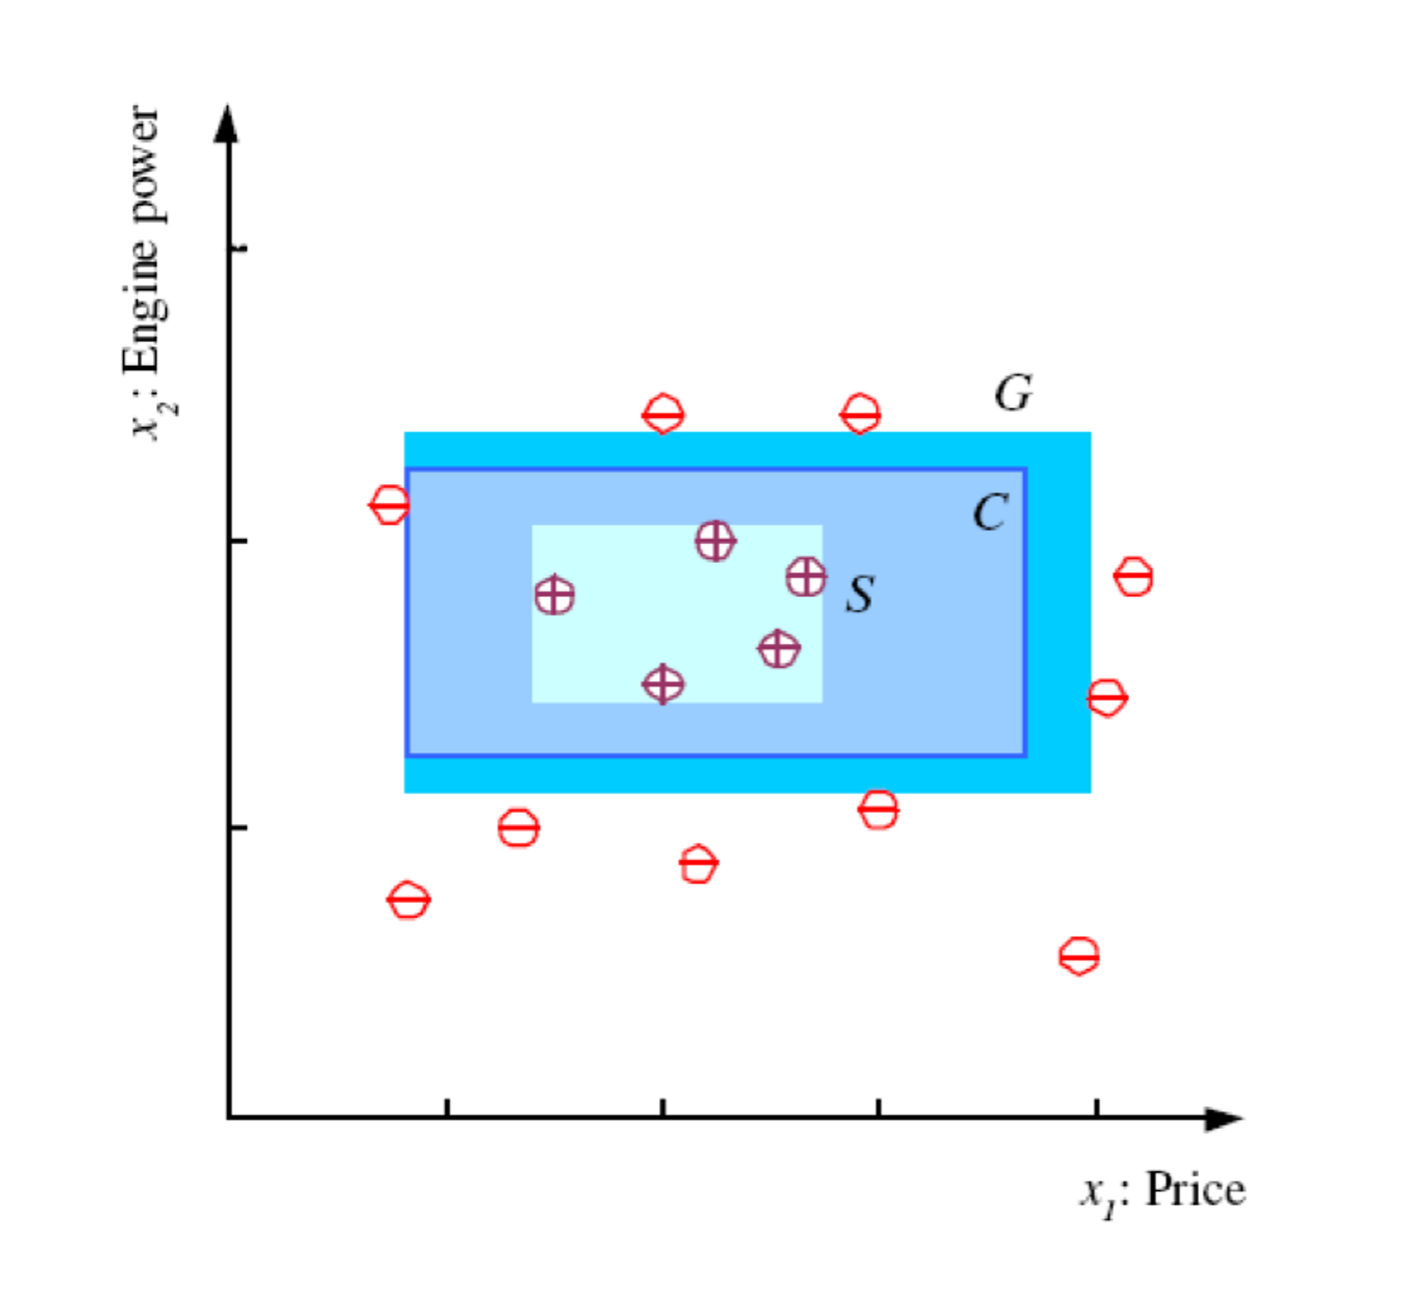
\includegraphics[width=0.5\columnwidth]{images/version-space.png}
    \caption{Illustration of a Version Space.}
    \label{fig:fig2}
\end{figure}

\begin{itemize}
\itemsep1pt\parskip0pt\parsep0pt
\item
  Intuitively, the \textbf{''safest'' hypothesis} to choose from the
  version space is the one that is furthers from the positive and
  negative training examples $\rightarrow$ maximum margin

  \begin{itemize}
  \itemsep1pt\parskip0pt\parsep0pt
  \item
    Margin = minimum distance between the decision boundary and a
    training point
  \end{itemize}
\end{itemize}






\subsection{Regression (Task 2/3) }\label{regression}

\textbf{Problem:} output variables which are numeric.





\subsection{Ranking \& preference learning (Task 3/3)
}\label{ranking-preference-learning}

\textbf{Problem:} predict a ordered list of preferred objects.

\textbf{Training data (typically):} pairwise preferences.

\begin{itemize}
  \item e.g.~user $x$ prefers movie $y_i$ over movie $y_j$
\end{itemize}

\textbf{Output:} ranked list of elements.




\subsection{Generalization}\label{generalization}

\textbf{Aim:} predict as well as possible the outputs of future
examples, not only for training sample.

We would like to \emph{minimize} the \textbf{generalization error}, or
the \textbf{(true) risk}:

\begin{equation} \label{eq:1}
  R(h) = E_{(x,y) \sim D}[L(h(x), y)]
\end{equation}
\begin{gather*}
  \text{Where:} \\
  \textbf{D}: \text{\underline{Unknown} distribution where from training and future} \\ \text{examples are drawn from (\underline{i.i.d assumption})}
\end{gather*}

\textbf{What can we say about $R(h)$} based on training examples and the
hypothesis class H alone? \underline{Two possibilities}:

\begin{itemize}
  \item Empirical evaluation by testing (Section \ref{model-evaluation-by-testing})
  \item Statistical learning theory (Section \ref{statistical-learning-theory})
\end{itemize}






\subsubsection{Model evaluation by testing
}\label{model-evaluation-by-testing}

\textbf{What:} estimate the model's ability to generalize on future data

\textbf{How:} approximating true risk by computing the
empirical risk on a independent test sample:

\[R_{test}(h) = \sum_{(x_i,y_i) \in S_{test}}^{m} L(h(x_i),y_i)\]

\begin{itemize}
  \item The expectation of $R_{test}(h)$ is the true risk $R(h)$
\end{itemize}





\subsection{Hypothesis classes }\label{hypothesis-classes}

There is a huge number of different \textbf{\textcolor{blue}{hypothesis classes}} or
\textbf{\textcolor{blue}{model families}} in machine learning, \textbf{e.g:}

\begin{itemize}
  \item
    \textbf{Linear models} such as logistic regression and perceptron
  \item
    \textbf{Neural networks:} compute non-linear input-output mappings
    through a network of simple computation units
  \item
    \textbf{Kernel methods:} implicitly compute non-linear mappings into
    high-dimensional feature spaces (e.g.~SVMs)
  \item
    \textbf{Ensemble methods:} combine simpler models into powerful
    combined models (e.g.~Random Forests)
\end{itemize}

Each have their different pros and cons in different dimensions
(accuracy, efficiency, interpretability); No single best hypothesis
class exists that would be superior to all others in all circumstances

\begin{center}\rule{3in}{0.4pt}\end{center}

\section{Statistical Learning Theory
}\label{statistical-learning-theory}

\textbf{What:} Theoretical background on machine learning.

\textbf{Goal:} Generalization (Section \ref{generalization})

\subsection{Probably Approximately Correct (PAC) learning
}\label{probably-approximately-correct-pac-learning}

\textbf{What:} \emph{Theoretical framework} that formalizes the notion
of generalization in machine learning.

\textbf{Ingredients:}

\begin{itemize}
  \item
  \textbf{input space $X$} containing all possible
  \item
  \textbf{inputs $x$} * set of possible \textbf{labels $Y$} $($in binary
  classification $Y = \{0, 1\}$$)$
\end{itemize}

\textbf{Goal:} to learn a hypothesis with a low generalization error

\[R(h) = E_{x \sim D} [L_{0/1}(h(x), C(x))] = Pr_{x \sim D} (h(x) \neq C(x))\]


\end{document}
